It is important that any image is fed into the network crop by crop, meaning that for each crop there is a separate embedding. In this section crops embeddings were not combined in any way together and were analysed separately. However, it is strongly recommended for a further research to evaluate all the experiments by finding projections in a lower-dimensional space not only of separate crops, but of the image as a whole. For example, by simply averaging embeddings for all crops from the same image. In all experiments here a model trained on nuclei dataset was used.

The UNet embedding has a size of $16 \times 16 \times 256$ and can be flattened into a $655536$-dimensional vector. In order to comprehend the embeddings for us as humans, a dimensionality reduction algorithm has to be applied. One option would be to compress a vector to 2D or 3D representation, which is easily comprehendable by humans.
\begin{figure}[htb]
	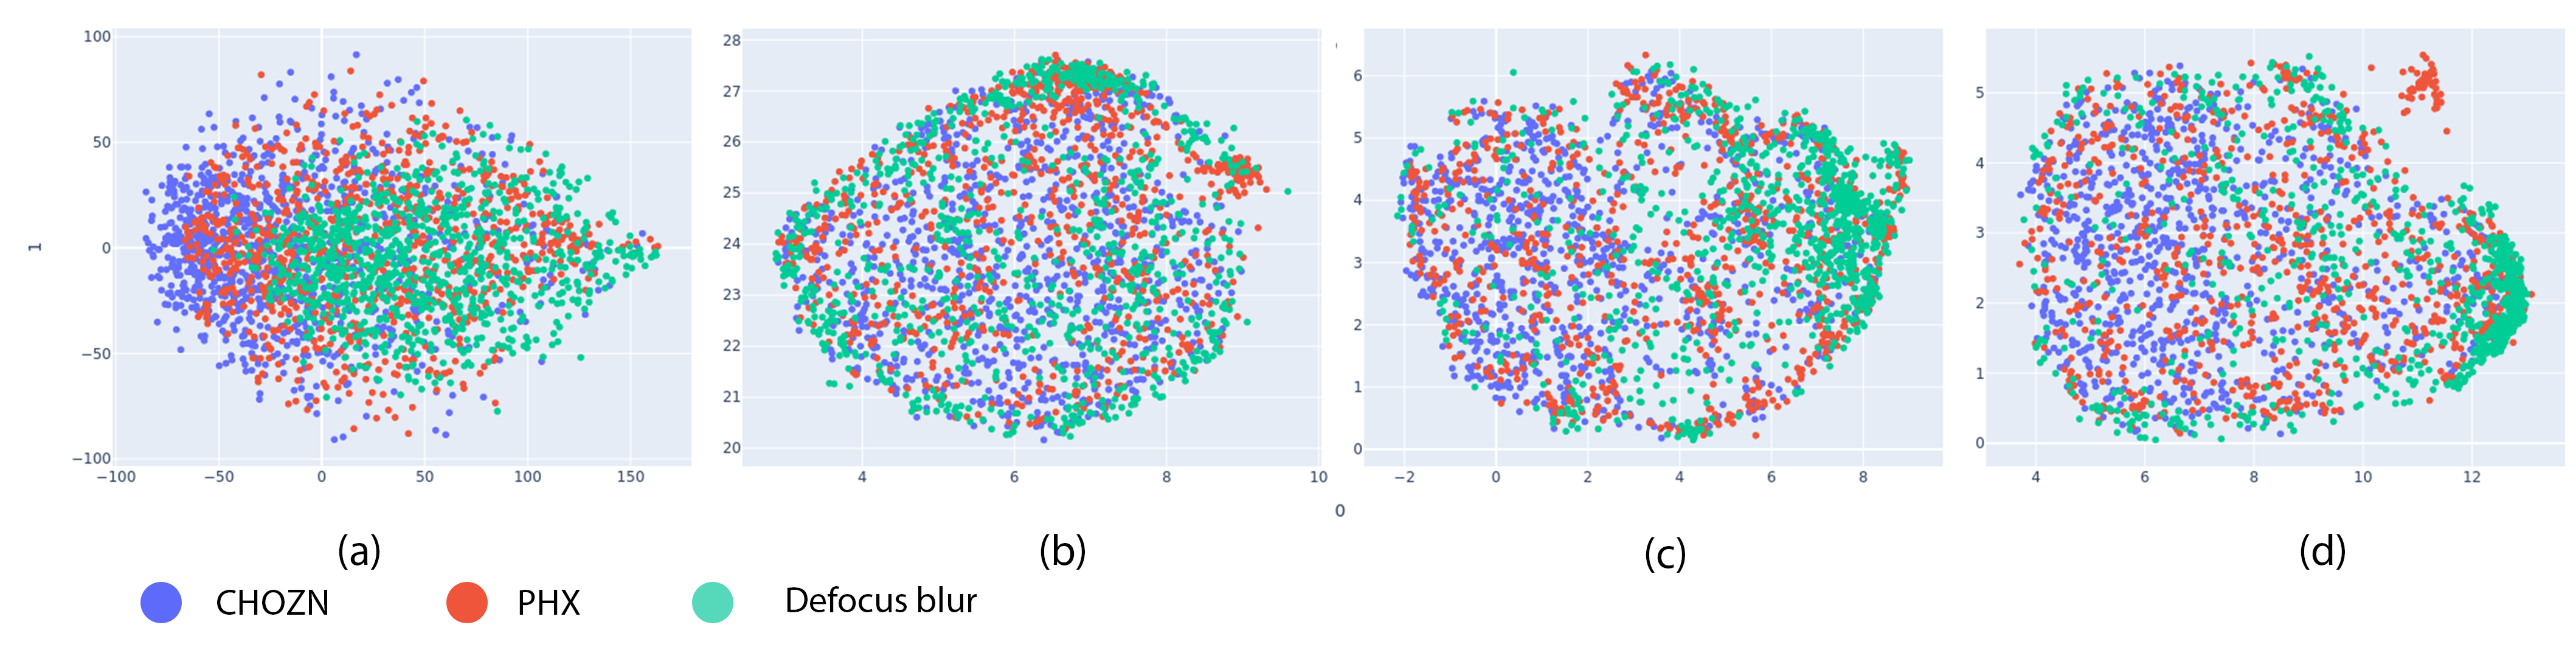
\includegraphics[width=\linewidth]{bilder/unet-embeddings/umap-pca-embeddings.png}
	\caption{(a) PCA, (b) UMAP, (c) combination of PCA and UMAP with 10 and (d) 50 components}\label{fig:umap-pca-embeddings}
\end{figure}

In this case a two-dimensional representation was chosen. With the help of PCA, UMAP and their combination embeddings were projected into a 2D space. In Figure \ref{fig:umap-pca-embeddings} we can see the clouds of dots, where each dot represents a projected UNet embedding of a crop. Both research questions are addressed here: clustering based on phenotypes (CHOZN or PHX) and clustering based on input corruptions (defocus blur of severity level $4$). It is crucial here that corrupted data was not used in training of any of dimensionality reduction method. The goal was to use only the data available in training dataset, find the transformation of high-dimensional data into a lower-dimensional space and apply it to new samples. That is also why methods like t-sne \cite{t-sne} cannot be used here, because the transformation that t-sne learns cannot be applied to new samples. 

From Figure \ref{fig:umap-pca-embeddings} it becomes evident that there is no clustering based on the phenotype. On the one hand, this means that it is not possible to detect phenotype based on the UNet embedding. But on the other hand, this also implies that PHX or CHOZn phenotypes do not influence the predictions so much supports previous conclusion from Section \ref{section:generalizability-across-phenotypes} that the model generalises well across them. 

In the Figure \ref{fig:umap-pca-embeddings} green corrupted dots seem to clump more in groups, occupying either one side (a, d) or the area around the center (b). It is also clear that the combination of UMAP with previously applied PCA works better with the increasing amount of components in PCA: dots in (d) seem to form a better cluster than dots in (c). However, it can still not be taken intuitively from this figure how many non-corrupted dots are hidden behind the cluster of the green dots --- meaning whether non-corrupted crops cluster intersects severely with a corrupted one. In order to visualize this better, one can use a kernel density estimate (KDE) plot presented in Figure \ref{fig:kde}. Additionally, it is clear that pure UMAP is not the best approach for the extreme number of dimensions as with the one in this case.

\begin{figure}[htb]
	\begin{center}
		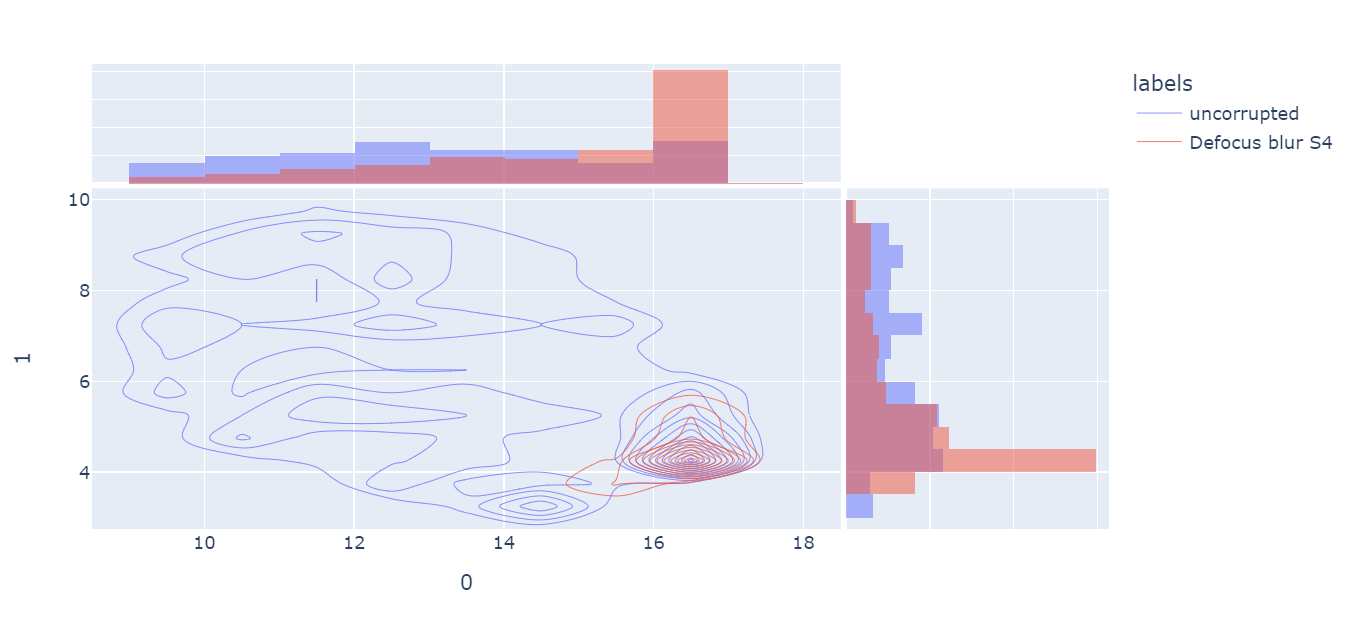
\includegraphics[width=0.6\linewidth]{bilder/unet-embeddings/kde.png}
	\caption{KDE plot of UMAP applied after PCA with 200 components}\label{fig:kde}
	\end{center}
\end{figure}

A cluster of corrupted images is clearly present here, however it also intersects with many non-corrupted crops. The quantitative evaluation of how this cluster is separable from the rest of the points is provided in section \ref{section:clustering-on-unet-embeddings}. Although one can already state that there is a clear opportunity to differentiate between corrupted and not corrupted images, the accuracy cannot be high due to the clusters being not well separable. For further research it is suggested to additionally check whether clusters form into a high-dimensional space before projecting them into a 2D space. 
